
Throughout this first section, our main focus is to:
\begin{enumerate}
    \item Effectively load and store the data in a \texttt{Pandas} DataFrame for subsequent processing
    \item Analyze the distribution of the target labels and features to design the preprocessing strategy to be followed accordingly
\end{enumerate}

% ------------------------------------------------------
\section{Loading the Dataset and Libraries}

Throughout the project, \texttt{Pandas} and \texttt{Numpy} libraries are utilized for data wrangling and numerical functionalities on data, \texttt{Matplotlib} and \texttt{Seaborn} are jointly used for data visualization, and \texttt{tqdm} was employed to display a progress bar during each training process. However, due to rise of performance issues, we disregarded the use of \texttt{tqdm} in the project later.

Moreover, we attempted to load the dataset directly from the provided Google Drive link~\cite{dataset} associated with the project. The dataset comprises 10 features, denoted as $x_1, \dots, x_{10}$, and contains \texttt{10,000} samples in total. Using the \texttt{info()} function from \texttt{Pandas}, it was confirmed that there are no missing values, as all features have a complete set of \texttt{10,000} samples.

Upon analyzing the dataset, we observed the following:
\begin{itemize}
    \item The feature matrix $X$ consists exclusively of numerical values, eliminating the need for any conversion from categorical to numerical data. All features are stored as \texttt{float64}, so no data type conversion is required.
    \item The target labels $y$ are binary, taking values from the set $\{-1, 1\}$. These labels are stored as \texttt{int64}, which aligns well with our classification objectives.
\end{itemize}

% ------------------------------------------------------
\section{Data Distribution Exploration}

Analyzing the distribution of target labels $y$ using the \texttt{value\_counts()} function on the DataFrame reveals that the dataset is almost perfectly \textit{balanced}, with roughly the same number of positive and negative classes distributed among the samples of the dataset (\texttt{5,008} negative and \texttt{4,992} positive). Figure~\ref{fig:distribution_targets} illustrates this distribution.

\begin{figure}[h]
    \centering
    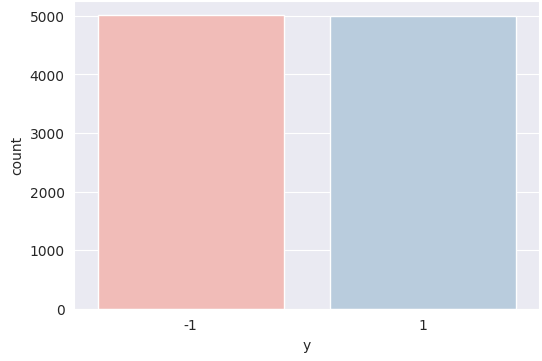
\includegraphics[width=0.6\linewidth]{distribution_targets.png}
    \caption{Distribution of Target Labels}
    \label{fig:distribution_targets}
\end{figure}

On the other hand, analyzing the distribution of features $x_i \in \mathcal{X}$ using the \texttt{describe()} function, it can be seen that the range of values each feature takes is different than the other. Consequently, we need to apply appropriate scaling methods during preprocessing to ensure that features with larger value ranges do not dominate the influence on our predictions. These different distributions are visualized in Figure~\ref{fig:distribution_features}.

\begin{figure}[h]
    \centering
    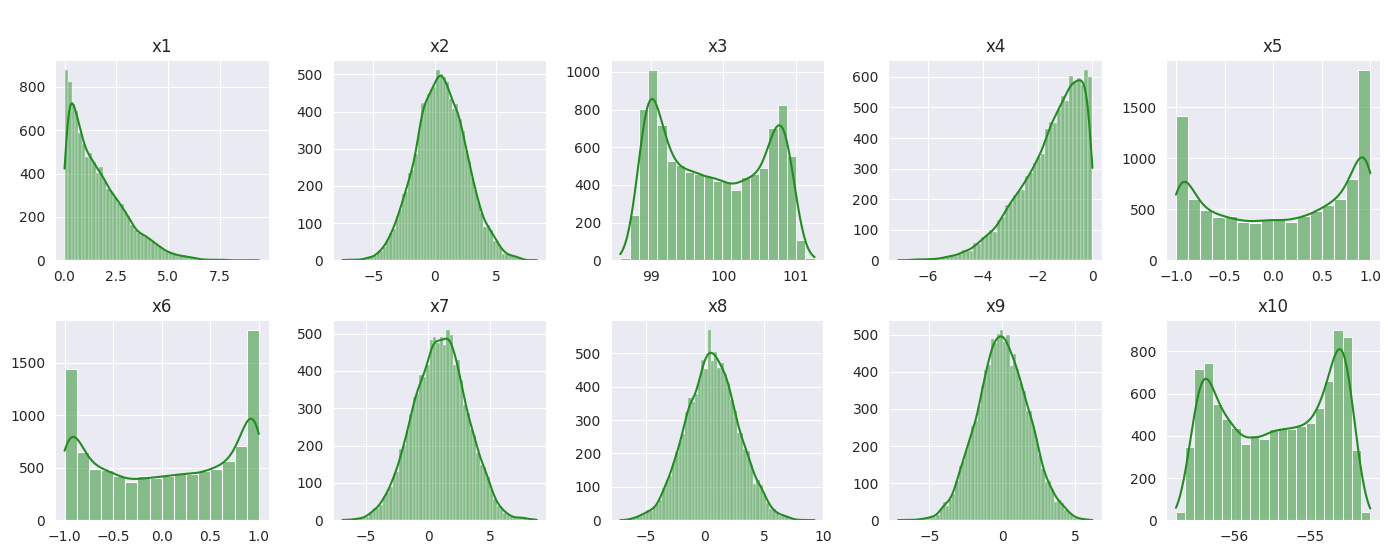
\includegraphics[width=\linewidth]{images/distribution_features.png}
    \caption{Distribution of Features}
    \label{fig:distribution_features}
\end{figure}

Additionally, we will assess the potential presence of noise and outliers. While techniques such as the \textit{z-score} are available for outlier detection, we will first examine the boxplot for each feature. Subsequently, we will use the Interquartile Range (IQR) method to establish outlier boundaries and remove them, as it is widely recognized and reliable in the field.

The IQR measures the spread of the central \texttt{50\%} of a dataset by calculating the difference between the third quartile (Q3) and the first quartile (Q1), given by:
\begin{equation}
    \text{IQR} = Q3 - Q1
\end{equation}

To identify outliers, we compute the lower and upper bounds as follows, where the data points outside these bounds are considered potential outliers:
\begin{equation}
    \text{Lower Bound} = Q1 - 1.5 \times \text{IQR}
\end{equation}
\begin{equation}
    \text{Upper Bound} = Q3 + 1.5 \times \text{IQR}
\end{equation}

The IQR method is effective in identifying the impact of outliers, thereby improving the accuracy of our dataset analysis. As it is illustrated in Figure~\ref{fig:outlier_removal}, the majority of outliers have been addressed using the IQR technique, allowing us to proceed to the next step. Following outlier removal, the dataset now includes \texttt{9,456} samples, indicating that approximately \texttt{550} samples were removed.

\begin{figure}[h]
     \centering
     \begin{subfigure}[b]{0.45\textwidth}
         \centering
         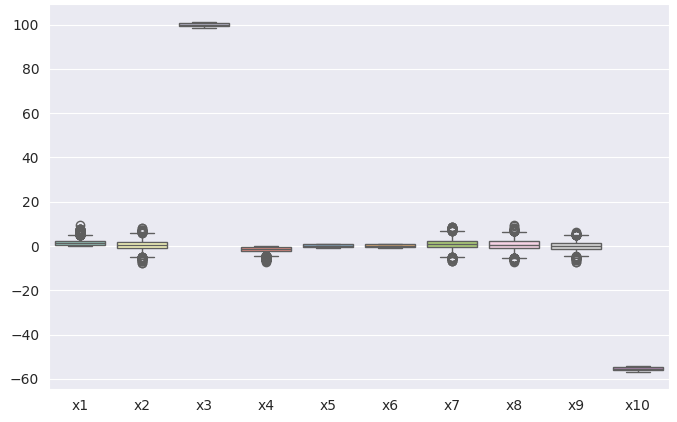
\includegraphics[width=\textwidth]{images/outliers_before.png}
         \caption{Before outlier removal}
         \label{fig:outliers_before}
     \end{subfigure}
     \hfill
     \begin{subfigure}[b]{0.45\textwidth}
         \centering
         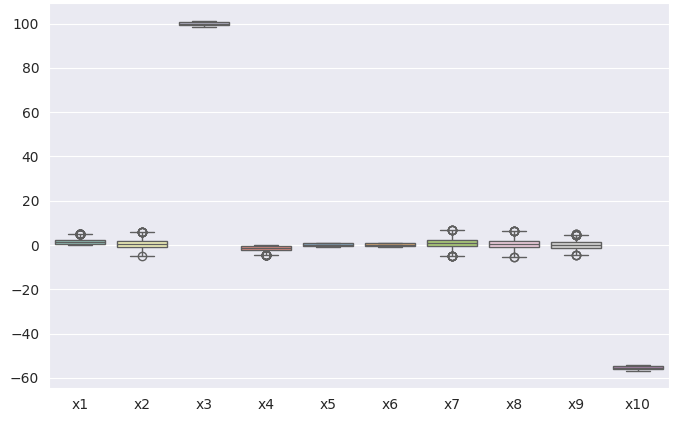
\includegraphics[width=\textwidth]{images/outliers_after.png}
         \caption{After outlier removal}
         \label{fig:outliers_after}
     \end{subfigure}
     
    \caption{Box-plots of different features and the effect of outlier removal}
    \label{fig:outlier_removal}
\end{figure}

This method, however, may not eliminate all data points that are distant from the majority of the data. Some points, although not classified as extreme outliers, may still be noticeably separated from the main cluster of data and can appear as mild outliers in the boxplot.
